\documentclass[11pt,a4paper]{article}

% --- Essential Packages ---
\usepackage[utf8]{inputenc}
\usepackage[vietnamese]{babel}
\usepackage[top=1.8cm, bottom=2.0cm, left=2.0cm, right=2.0cm]{geometry}
\usepackage{amsmath, amssymb, amsfonts, amsthm, mathtools}
\usepackage{graphicx}
\usepackage{float}
\usepackage{subcaption}
\usepackage{booktabs, multirow, makecell}
\usepackage{algorithm, algpseudocode}
\usepackage{siunitx}
\usepackage[table]{xcolor}
\usepackage{cite}
\usepackage{microtype}
\usepackage{enumitem}
\usepackage{tabularx}
\usepackage{tcolorbox}
\usepackage{tikz}
\usepackage{titlesec}
\usepackage[colorlinks=true, linkcolor=blue!70!black, citecolor=red!70!black, urlcolor=blue!70!black]{hyperref}

% --- Color Definitions matching template ---
\definecolor{bannerbg}{HTML}{EBE3E0}      % Soft pastel taupe/rose banner
\definecolor{logobg}{HTML}{222222}        % Dark charcoal square logo
\definecolor{linecolor}{HTML}{D0C8C6}      % Subtle divider line
\definecolor{tableheader}{HTML}{F5F5F5}   % Soft gray table header
\definecolor{rulecolor}{HTML}{DDDDDD}     % Table grid rule

% --- Section Formatting matching template ---
\titleformat{\section}{\large\bfseries\color{black}}{}{0em}{}[\vspace{0.15cm}]
\titlespacing*{\section}{0pt}{1.2ex plus .2ex minus .2ex}{0.8ex plus .1ex minus .1ex}

\titleformat{\subsection}{\normalsize\bfseries\color{black}}{}{0em}{}
\titlespacing*{\subsection}{0pt}{1.0ex plus .2ex minus .1ex}{0.5ex plus .1ex minus .1ex}

% Custom section divider line
\newcommand{\sectiondivider}{\vspace{0.25cm}\noindent{\color{linecolor}\rule{\textwidth}{0.6pt}}\vspace{0.25cm}}

% Theorem and algorithm Vietnamese definitions
\newtheorem{theorem}{Định lý}
\newtheorem{lemma}{Bổ đề}
\floatname{algorithm}{Thuật toán}
\renewcommand{\algorithmicrequire}{\textbf{Đầu vào:}}
\renewcommand{\algorithmicensure}{\textbf{Đầu ra:}}

\setlength{\parindent}{0pt}
\setlength{\parskip}{5pt}
\linespread{1.12}

\begin{document}

% =========================================================================
% TOP HEADER BANNER (Matching Template Style)
% =========================================================================
\noindent
\begin{minipage}[t]{0.75\textwidth}
    \textbf{Posts and Telecommunications Institute of Technology (PTIT)}\\
    \textbf{Faculty of Telecommunications II}\\[0.12cm]
    \small \textbf{Email:} \texttt{nmquan3108@gmail.com}
\end{minipage}%
\hfill

\vspace{0.25cm}
\hrule height 0.8pt
\vspace{0.8cm}

% =========================================================================
% DOCUMENT TITLE (Matching Template Style)
% =========================================================================
\begin{center}
    {\LARGE \textbf{Tối ưu hóa Đồng thời Quỹ đạo bay và Phân bổ Công suất trong Mạng SAGIN-NOMA:}\\[0.1cm]
    \textbf{Từ Tối ưu hóa Luân phiên (AO) đến Học tăng cường sâu (DRL) Thời gian thực}}\\[0.25cm]
\end{center}

\vspace{0.2cm}
\noindent{\color{linecolor}\rule{\textwidth}{0.6pt}}
\vspace{0.3cm}

% =========================================================================
% MODULAR CONTENT SECTIONS
% =========================================================================
\section*{I. Tóm tắt Thực thi}

Báo cáo này cung cấp phân tích định lượng về quy trình tối ưu hóa mạng tích hợp Không gian - Trên không - Mặt đất hỗ trợ Đa truy nhập phi trực giao (SAGIN-NOMA). Mục tiêu cốt lõi của nghiên cứu là cực tiểu hóa xác suất dừng toàn phần ($P_{\text{out}}$) của hệ thống, nâng cao độ tin cậy dịch vụ trên kênh fading Rician tổng quát, đồng thời bảo đảm tính khả thi nghiêm ngặt của kỹ thuật Khử nhiễu liên tiếp (SIC). Báo cáo trình bày chi tiết mô hình hệ thống hai chặng (Vệ tinh $\to$ Cụm tiếp sóng UAV với cơ chế PRS $\to$ Hai người dùng mặt đất), dẫn giải giải tích dạng đóng chính xác qua hàm Marcum-Q, cùng hai phương pháp tối ưu hóa: (i) Tối ưu hóa Luân phiên (Alternating Optimization - AO) số học đóng vai trò nghiệm tham chiếu chuẩn (Benchmark); và (ii) Tác tử Học tăng cường sâu (Deep Reinforcement Learning - DRL) tùy biến theo kiến trúc Actor-Critic cho phép ra quyết định điều khiển quỹ đạo bay và phân bổ công suất trực tuyến ở cấp độ mili-giây. Các kết quả thực nghiệm mô phỏng, phân tích so sánh định lượng và các thông số kỹ thuật triển khai thực tế trên các nền tảng bay 6G được trình bày chi tiết trong báo cáo này.

\sectiondivider

\section*{II. Giới thiệu \& Bối cảnh}

\subsection*{Bối cảnh}
Mạng tích hợp Không gian - Trên không - Mặt đất (Space-Air-Ground Integrated Networks - SAGIN) được định vị là hạ tầng trụ cột của mạng không dây thế hệ thứ sáu (6G), nhằm xóa bỏ các điểm mù kết nối tại vùng sâu, vùng xa, hải đảo và hỗ trợ cứu hộ khẩn cấp \cite{liu2018space, zeng2019accessing}. Trong kiến trúc này, vệ tinh cung cấp vùng phủ sóng diện rộng nhưng chịu suy hao truyền sóng trong không gian tự do rất lớn. Việc tích hợp Phương tiện bay không người lái (UAV) đóng vai trò trạm tiếp sóng Giải mã và Chuyển tiếp (Decode-and-Forward - DF) giúp tái tạo tín hiệu, rút ngắn cự ly truyền thông và thiết lập kênh truyền tầm nhìn thẳng (LoS) thuận lợi \cite{wu2018joint}. Khi kết hợp với công nghệ Đa truy nhập phi trực giao (NOMA) phân chia miền công suất, UAV có thể phục vụ đồng thời nhiều người dùng mặt đất trên cùng một khối tài nguyên tần số - thời gian, nâng cao đáng kể hiệu quả sử dụng phổ tần \cite{ding2017survey}. Tuy nhiên, chuyển động linh hoạt của UAV đòi hỏi phải kiểm soát chặt chẽ ranh giới không gian nhằm tránh đảo lộn thứ tự giải mã khử can nhiễu liên tiếp (SIC), đặt ra một bài toán tối ưu hóa phi lồi phi tuyến phức tạp.

\subsection*{Mục tiêu Đề tài}
Đề tài tập trung giải quyết ba mục tiêu kỹ thuật cụ thể sau:
\begin{enumerate}[label=\textbf{\arabic*.}]
    \item \textbf{Dẫn giải Giải tích Chính xác:} Thiết lập biểu thức giải tích dạng đóng cho xác suất dừng (Outage Probability - OP) của từng người dùng và toàn hệ thống trên kênh fading Rician tổng quát thông qua hàm Marcum-Q bậc 1 \cite{alouini2001digital} có xét đến cơ chế Lựa chọn Chuyển tiếp Từng phần (PRS).
    \item \textbf{Thiết lập Nghiệm Tham chiếu Chuẩn (AO Benchmark):} Xây dựng khung Tối ưu hóa Luân phiên (AO) phân rã bài toán thành tối ưu quỹ đạo bay (bằng Sequential Quadratic Programming - SQP) và phân bổ công suất (bằng Golden Section Search) dưới các ràng buộc động học và ranh giới hình học SIC.
    \item \textbf{Hiện thực hóa Điều khiển Thời gian thực (Real-Time DRL):} Thiết kế và huấn luyện mạng Actor-Critic liên tục dựa trên thuật toán Deep Deterministic Policy Gradient (DDPG) \cite{lillicrap2015continuous} với kỹ thuật Dịch chuyển Định hướng (Guided Displacement) và Nạp mồi Khởi tạo (Warm-Start Seeding), đạt thời gian suy luận $\approx 1.5$ ms/khe phục vụ điều khiển bay trực tuyến thích ứng.
\end{enumerate}

\sectiondivider

\section*{III. Phương pháp luận \& Mô hình Kỹ thuật}

\subsection*{Tổng quan Hệ thống}
Hệ thống mạng SAGIN-NOMA được mô hình hóa trên mặt phẳng tọa độ 2D chuẩn hóa $(Oxz)$ với các thành phần và tham số vật lý:
\begin{itemize}[leftmargin=1.5em]
    \item \textbf{Kiến trúc Không gian - Thời gian:} Một vệ tinh nguồn $S$ tại tọa độ chuẩn hóa $\mathbf{q}_S = (0.0, 1.0)$ (mô hình hình học chuẩn hóa 2D mang tính minh họa với cự ly quy đổi $D_0 = 125$ m); một cụm gồm $N_{\text{UAV}} = 3$ trạm tiếp sóng UAV bay theo đội hình cụm lân cận (cluster) quanh vị trí danh định $\mathbf{q}_U[n]$ (cơ chế PRS chọn UAV có độ lợi kênh tức thời tốt nhất trong cụm); và hai người dùng mặt đất gồm người dùng gần $D_2$ tại $\mathbf{q}_{D2} = (1.0, 0.0)$ và người dùng xa $D_1$ tại $\mathbf{q}_{D1} = (1.5, 0.0)$. Hành trình bay của UAV được chia thành $N = 10$ khe thời gian rời rạc, mỗi khe kéo dài $dt = 2.0$ giây (tổng thời gian hành trình $T = 20.0$ s).
    \item \textbf{Chuẩn hóa Kích thước \& Vận tốc:} Khoảng cách được chuẩn hóa theo hệ số $D_0 = 125$ m (1 đơn vị chuẩn hóa tương đương $125$ m thực địa). Vận tốc bay cực đại $V_{\max} = 15$ m/s tương ứng với độ dịch chuyển chuẩn hóa tối đa mỗi khe là $\Delta d_{\max} = V_{\max} \cdot dt / D_0 = 15 \times 2 / 125 = 0.24$ đơn vị.
    \item \textbf{Mô hình Kênh Fading Rician:} Cả hai chặng truyền thông đều chịu ảnh hưởng của fading Rician tổng quát kết hợp suy hao đường truyền theo khoảng cách Euclidean với số mũ suy hao $\nu_{SU} = 2.0$ (chặng 1) và $\nu_{UD} = 2.2$ (chặng 2). Hệ số Rician lần lượt là $K_{SU} = 5.0$ (thành phần LoS vệ tinh chiếm ưu thế) và $K_{UD} = 3.0$.
    \item \textbf{Cơ chế PRS và Ghép mã NOMA:} Chặng 1 áp dụng cơ chế Lựa chọn Chuyển tiếp Từng phần (PRS), trong đó UAV có độ lợi kênh $|h_{SU_k}|^2$ lớn nhất trong cụm $N_{\text{UAV}} = 3$ được chọn để giải mã tín hiệu từ vệ tinh. Tại chặng 2, UAV được chọn phát đồng thời tín hiệu tới $D_1, D_2$ theo nguyên lý NOMA phân chia miền công suất với $\alpha_1[n] + \alpha_2[n] = 1$ ($\alpha_1[n] > \alpha_2[n]$). Người dùng gần $D_2$ tiến hành giải mã khử nhiễu liên tiếp (SIC) tín hiệu của $D_1$ trước khi tách tín hiệu của chính mình.
\end{itemize}

\subsection*{Thiết lập Bài toán Tối ưu hóa}
Để cực tiểu hóa xác suất dừng trung bình toàn mạng $\bar{P}_{\text{out}}$ trên toàn bộ hành trình $N = 10$ khe, bài toán tối ưu hóa liên hợp giữa chuỗi tọa độ quỹ đạo bay $\mathbf{Q} \in \mathbb{R}^{N \times 2}$ và chuỗi vector công suất $\boldsymbol{\alpha}_1 \in \mathbb{R}^N$ được thiết lập như sau:
\begin{subequations}
\label{eq:opt_problem}
\begin{align}
    \min_{\mathbf{Q}, \, \boldsymbol{\alpha}_1} \quad & \bar{P}_{\text{out}} = \frac{1}{N} \sum_{n=1}^N OP_{\text{total}}[n] \label{eq:obj} \\
    \text{thỏa mãn} \quad 
    & \text{C1}: x_{\min} \le x_U[n] \le x_{\max}, \quad z_{\min} \le z_U[n] \le z_{\max}, \quad \forall n \in \{1, \dots, N\}, \label{eq:c1} \\
    & \text{C2}: \mathbf{q}_U[1] = \mathbf{q}_{\text{start}} = (0.35, 0.50), \quad \mathbf{q}_U[N] = \mathbf{q}_{\text{end}} = (1.10, 0.30), \label{eq:c2} \\
    & \text{C3}: \|\mathbf{q}_U[n] - \mathbf{q}_U[n-1]\| \le \Delta d_{\max} = 0.24, \quad \forall n \in \{2, \dots, N\}, \label{eq:c3} \\
    & \text{C4}: x_U[n] \le \frac{x_{D1} + x_{D2}}{2} - \Delta_{\text{margin}} = 1.21, \quad \forall n, \label{eq:c4} \\
    & \text{C5}: \alpha_1[n] + \alpha_2[n] = 1, \quad \forall n, \label{eq:c5} \\
    & \text{C6}: \alpha_1[n] \ge \alpha_{1,\min} = \frac{\gamma_{th1}}{1 + \gamma_{th1}} \approx 0.670, \quad \alpha_1[n] \le 1 - \epsilon_{\text{sic}}, \quad \forall n. \label{eq:c6}
\end{align}
\end{subequations}
Trong đó ràng buộc $\text{C1}$ quy định hành lang bay an toàn $x \in [0.10, 1.30]$ và $z \in [0.20, 0.60]$; $\text{C2}$ cố định điểm bắt đầu và điểm kết thúc hành trình; $\text{C3}$ là ràng buộc động học bước bay tối đa; $\text{C4}$ là \textbf{ràng buộc ranh giới hình học SIC} bảo đảm điều kiện suy hao cự ly trung bình $d_{UD2}[n] < d_{UD1}[n]$ luôn thỏa mãn nhằm duy trì trật tự giải mã SIC; $\text{C5}$ và $\text{C6}$ bảo đảm bảo toàn công suất phát và ngưỡng khả thi cho quá trình giải mã SIC tại $D_2$.

\subsection*{Phương pháp Giải thuật Tối ưu}
Do bài toán \eqref{eq:opt_problem} có tính chất phi lồi (non-convex) và chứa hàm giải tích Marcum-Q phi tuyến phức tạp, nghiên cứu triển khai hai giải pháp đối sánh:
\begin{enumerate}[label=\textbf{\arabic*.}]
    \item \textbf{Tối ưu hóa Luân phiên Tĩnh (Static AO Benchmark):} Khảo sát tại một vị trí snapshot danh định để phân tích đặc tính hội tụ của giải thuật lặp luân phiên giữa tọa độ UAV và cặp công suất $(\alpha_1, \alpha_2)$, đồng thời kiểm chứng tính chính xác của biểu thức giải tích qua so sánh với mô phỏng thống kê Monte-Carlo.
    \item \textbf{Tối ưu hóa Luân phiên Động (Dynamic Time-Slotted AO):} Mở rộng trên toàn bộ $N=10$ khe thời gian, kết hợp giải thuật Quy hoạch toàn phương tuần tự (SQP) cho biến quỹ đạo và Tìm kiếm lát cắt vàng cho biến công suất. Do bài toán phi lồi, nghiệm của AO đóng vai trò là \textbf{nghiệm tham chiếu chuẩn (Numerical Benchmark)} giúp đánh giá hiệu năng của các giải thuật khác.
    \item \textbf{Học tăng cường sâu Thời gian thực (Real-Time DRL Agent):} Xây dựng mạng nơ-ron Actor-Critic liên tục \cite{lillicrap2015continuous}. Trạng thái tại khe $n$ bao gồm vị trí hiện tại, khoảng cách tới các nút và biên an toàn SIC: $\mathbf{s}_n = [x_n, z_n, d_{UD1}, d_{UD2}, d_{US}, \Delta_{\text{target}}, d_{\text{sic\_margin}}]^T$. Hành động gồm bước dịch chuyển vận tốc, góc bay và hệ số công suất: $\mathbf{a}_n = [v_n, \theta_n, \alpha_1[n]]^T$. Hàm phần thưởng logarit $R_n = -\ln(OP_{\text{total}}[n] + 10^{-6}) - P_{\text{penalty}}$ được định hình để dẫn hướng tác tử tối ưu hóa tức thời mà không bị triệt tiêu gradient.
\end{enumerate}

\sectiondivider

\section*{IV. Kết quả Thực nghiệm \& Đối chuẩn}

\subsection*{Bảng Chỉ số Hiệu năng Đối chuẩn Toàn diện}
Bảng dưới đây tổng hợp và đối chuẩn chi tiết các chỉ số hiệu năng cốt lõi giữa hai cấp độ mô hình: \textbf{Snapshot Tĩnh} (khảo sát tại tọa độ danh định $q_U^{(0)} = (0.5, 0.4)$) và \textbf{Hành trình Động học} ($N=10$ khe thời gian). Các mốc cơ sở (Baseline) được phân định rõ ràng nhằm phản ánh chính xác tỷ lệ cải thiện hiệu năng:

\vspace{0.2cm}
\begin{center}
\renewcommand{\arraystretch}{1.25}
\begin{tabularx}{\textwidth}{|X|>{\centering\arraybackslash}m{2.3cm}|>{\centering\arraybackslash}m{2.3cm}|>{\centering\arraybackslash}m{2.3cm}|>{\centering\arraybackslash}m{2.5cm}|}
\hline
\rowcolor{tableheader}
\textbf{Chỉ số Đánh giá (Metric)} & \textbf{Snapshot Tĩnh: AO Tĩnh} & \textbf{Hành trình Động: Trước Tối ưu} & \textbf{Hành trình Động: AO Động ($N=10$)} & \textbf{Hành trình Động: DRL DDPG} \\
\hline
Cấu hình không gian & Tọa độ tĩnh $q_U^{(0)}=(0.5, 0.4)$ & Quỹ đạo thẳng $q_{\text{start}} \to q_{\text{end}}$ & Tối ưu luân phiên SQP/Penalty & Học tăng cường Actor-Critic \\
Phân bổ công suất $\alpha_1$ & $\alpha_1^{(0)} = 0.75 \to 0.795$ & Cố định $\alpha_1 = 0.75$ & Động $\alpha_1^*[n] \in [0.77, 0.83]$ & Động $\alpha_1^*[n] \in [0.78, 0.83]$ \\
\hline
Xác suất dừng TB ($\bar{P}_{\text{out}}$) & $0.0701 \to \mathbf{0.00533}$ & $0.0401$ (BM3: $0.0481$) & $\mathbf{0.0206}$ & $\mathbf{0.0197}$ \\
Xác suất dừng xa $D_1$ & $0.0463 \to 0.00318$ & $0.0245$ & $0.0098$ & $0.0089$ \\
Xác suất dừng gần $D_2$ & $0.0249 \to 0.00216$ & $0.0160$ & $0.0109$ & $0.0110$ \\
\hline
Mức giảm xác suất dừng & \textbf{Giảm 92.4\%} (vs $0.0701$) & Baseline ($0\%$) & \textbf{Giảm 48.6\%} (BM3: $57.2\%$) & \textbf{Giảm 50.9\%} (BM3: $59.0\%$) \\
Thời gian tính toán / suy luận & $120.0$ ms & N/A & $1\,850.0$ ms (tổng 10 khe) & $\mathbf{1.5}$ \textbf{ms/khe} ($15$ ms tổng) \\
Số vòng lặp / tập hội tụ & $5$ vòng lặp & N/A & $4$ vòng lặp & $\approx 50$ episodes \\
Tỉ lệ vi phạm an toàn SIC & $\mathbf{0.0\%}$ (đệm an toàn) & $0.0\%$ (cố định) & $\mathbf{0.0\%}$ (đệm $0.10$) & $\mathbf{0.0\%}$ (đệm $0.06$) \\
Khả năng điều khiển trực tuyến & Ngoại tuyến & Không & Ngoại tuyến & \textbf{Trực tuyến (Real-time)} \\
\hline
\end{tabularx}
\end{center}
\vspace{0.2cm}

\subsection*{Quan sát Định lượng Cốt lõi}
\begin{itemize}[leftmargin=1.5em]
    \item \textbf{Phân định rõ ràng giữa hai mốc tham chiếu cơ sở (Baseline):} 
    (1) Đối với mô hình Snapshot Tĩnh tại tọa độ danh định $q_U^{(0)}=(0.5, 0.4)$ với $\alpha_1=0.75$, xác suất dừng trước tối ưu là $0.0701$, sau tối ưu giảm xuống $0.00533$ (mức suy giảm đạt $92.4\%$).
    (2) Đối với mô hình Hành trình Động qua $N=10$ khe thời gian, mốc trước tối ưu tương ứng với đường bay thẳng từ $q_{\text{start}}$ đến $q_{\text{end}}$ với công suất cố định $\alpha_1=0.75$ có xác suất dừng trung bình là $0.0401$ (hoặc $0.0481$ đối với kịch bản Benchmark 3 không tối ưu cả vị trí và công suất). Cả thuật toán AO Động và tác tử DRL đều giảm xác suất dừng về vùng xấp xỉ $\approx 0.02$ (AO đạt $0.0206$ - giảm $48.6\%$, DRL đạt $0.0197$ - giảm $50.9\%$).
    \item \textbf{Tính nhất quán toán học theo công thức dừng hệ thống:} Toàn bộ số liệu trong Bảng đều thỏa mãn nghiêm ngặt điều kiện xác suất dừng toàn phần $OP_{\text{total}} \ge \max(OP_{D1}, OP_{D2})$ theo đúng công thức xác suất hợp \eqref{eq:op_total_exact}.
    \item \textbf{Xác thực công thức giải tích Marcum-Q:} Kết quả mô phỏng Monte-Carlo với $10^5$ mẫu (ký hiệu hình tròn đen `ko' trên Hình \ref{fig:ao_static_snr}) phù hợp chặt chẽ với đường cong giải tích Marcum-Q trong phạm vi sai số thống kê cho phép trên toàn dải SNR từ $10 \to 26$ dB (tại $OP \approx 10^{-3}$, sai số thống kê lý thuyết của $10^5$ mẫu là khoảng $10\%$).
    \item \textbf{So sánh khách quan giữa DRL và AO theo quy ước khe thời gian:} 
    (1) \textit{Ảnh hưởng của quy ước khe:} Trong AO, quỹ đạo được tối ưu qua 10 nút mốc rời rạc với $q_1 = q_{\text{start}}$ và $q_{10} = q_{\text{end}}$ (tương ứng 9 bước di chuyển). Khe $n=1$ của AO được tính tại đúng điểm xuất phát $q_{\text{start}}(0.35, 0.50)$ cách xa người dùng nên $OP[1] \approx 0.1008$. Trong khi đó, tác tử DRL xuất phát tại $q_{\text{start}}$ ở $t=0$ và thực hiện 10 bước chuyển động, trong đó $OP[n]$ được tính sau mỗi bước (ở bước $n=1$, UAV đã dịch chuyển đến $(0.47, 0.435)$ gần người dùng hơn, dẫn đến $OP[1] \approx 0.0672$). Độ chênh lệch $\approx 0.0336$ tại khe 1 chia bình quân 10 khe đã đóng góp mức chênh lệch $\approx 0.0034$ vào xác suất dừng trung bình.
    (2) \textit{Hiệu năng tại các khe ổn định:} Tại các khe giữa ($n=5 \to 8$), giải thuật SQP của AO duy trì vị trí tối ưu ổn định ở $(1.105, 0.200)$ và đạt xác suất dừng $OP \approx 0.0053$, nhỉnh hơn so với mức $0.0056 - 0.0060$ của tác tử DRL. Điều này khẳng định AO đóng vai trò là cận tham chiếu chuẩn số học (numerical benchmark), trong khi DRL đạt hiệu năng bám sát cận chuẩn này.
    (3) \textit{Ưu thế quyết định của DRL:} Ưu thế then chốt của DRL nằm ở tốc độ suy luận trực tuyến $\mathbf{1.5}$ ms/khe (nhanh hơn $120$ lần so với thời gian giải lặp $1\,850$ ms của AO), cho phép triển khai điều khiển thời gian thực trên bo mạch UAV.
\end{itemize}

% -------------------------------------------------------------------------
\subsection*{1. Kết quả Mô phỏng Tối ưu hóa Luân phiên Tĩnh}
Mô hình AO Tĩnh thực hiện khảo sát tại một khe thời gian danh định (snapshot) nhằm kiểm chứng cơ sở toán học và đặc tính hội tụ cơ bản:

\begin{figure}[H]
    \centering
    \begin{subfigure}[b]{0.49\textwidth}
        \centering
        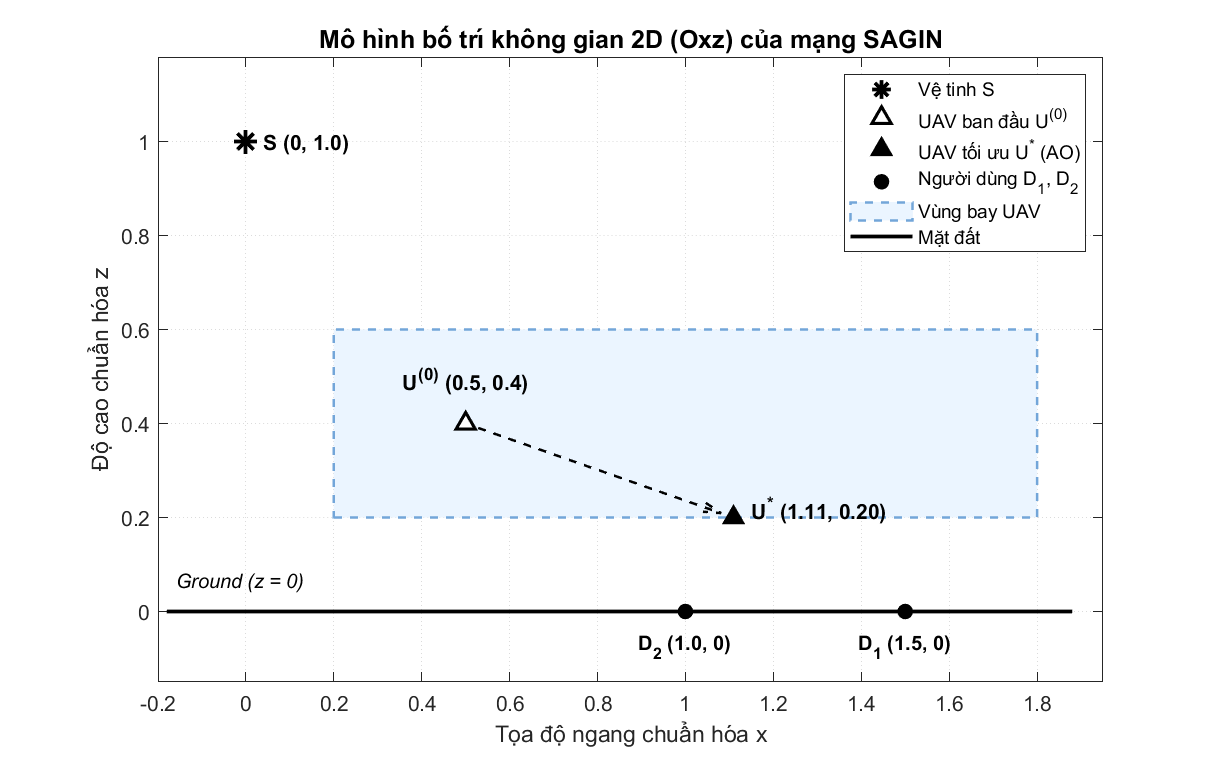
\includegraphics[width=\textwidth]{figures/ao_static_fig3_trajectory.png}
        \caption{Vị trí tĩnh tối ưu của UAV trong mặt phẳng 2D $(Oxz)$}
        \label{fig:ao_static_pos}
    \end{subfigure}
    \hfill
    \begin{subfigure}[b]{0.49\textwidth}
        \centering
        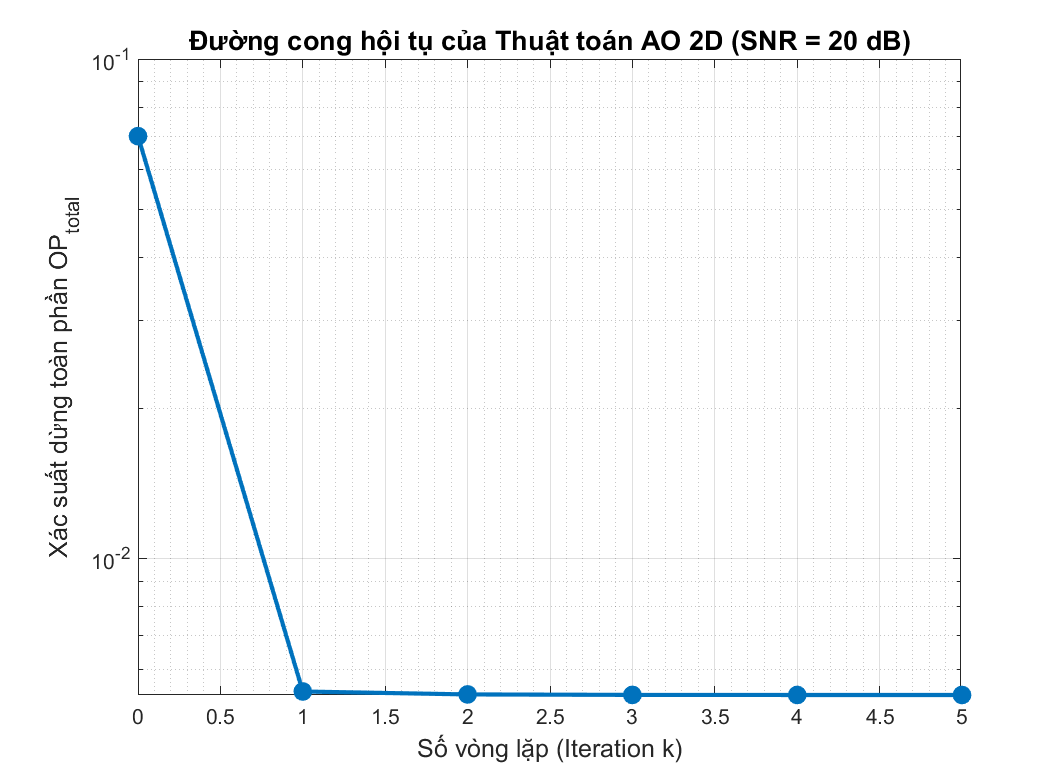
\includegraphics[width=\textwidth]{figures/ao_static_fig1_convergence.png}
        \caption{Đặc tính hội tụ của thuật toán AO tĩnh qua 5 vòng lặp}
        \label{fig:ao_static_conv}
    \end{subfigure}
    \caption{Kết quả vị trí không gian tĩnh và đặc tính hội tụ đơn điệu của giải thuật AO tĩnh.}
    \label{fig:ao_static_group1}
\end{figure}

\begin{figure}[H]
    \centering
    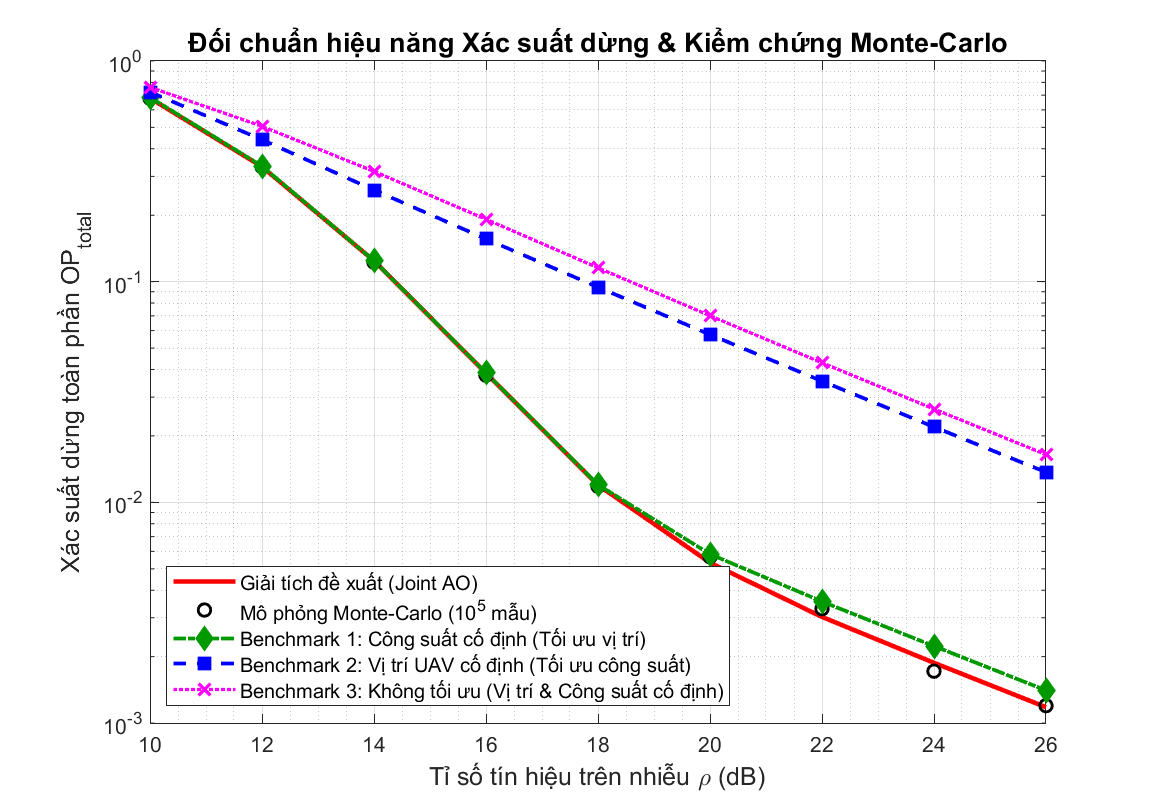
\includegraphics[width=0.72\textwidth]{figures/ao_static_fig2_snr.png}
    \caption{Đối chuẩn xác suất dừng qua dải SNR chuẩn hóa $\rho = \bar{\gamma}_S = \bar{\gamma}_U$ từ $10 \to 26$ dB: Kiểm chứng sự phù hợp giữa Mô phỏng Monte-Carlo ($10^5$ mẫu, ký hiệu dấu tròn `ko') và Biểu thức Giải tích hàm Marcum-Q bậc 1 (đường nét liền đỏ).}
    \label{fig:ao_static_snr}
\end{figure}

\begin{figure}[H]
    \centering
    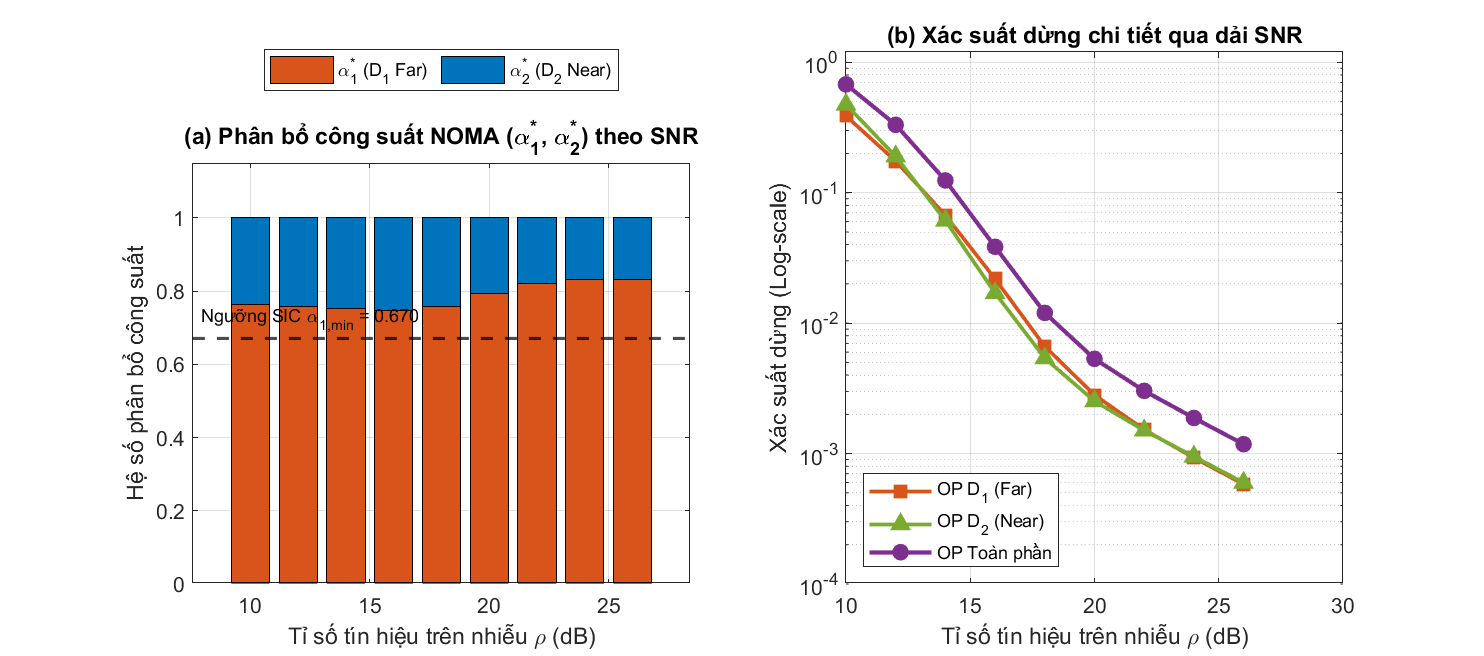
\includegraphics[width=0.86\textwidth]{figures/ao_static_fig4_power_outage.png}
    \caption{Phân bổ hệ số công suất NOMA ($\alpha_1^*, \alpha_2^*$) và xác suất dừng chi tiết từng người dùng qua dải SNR trong mô hình AO Tĩnh: (a) Phân bổ công suất NOMA với ngưỡng an toàn SIC $\alpha_{1,\min} = 0.670$; (b) Xác suất dừng chi tiết của người dùng xa $D_1$, người dùng gần $D_2$ và toàn phần hệ thống.}
    \label{fig:ao_static_power}
\end{figure}

\begin{figure}[H]
    \centering
    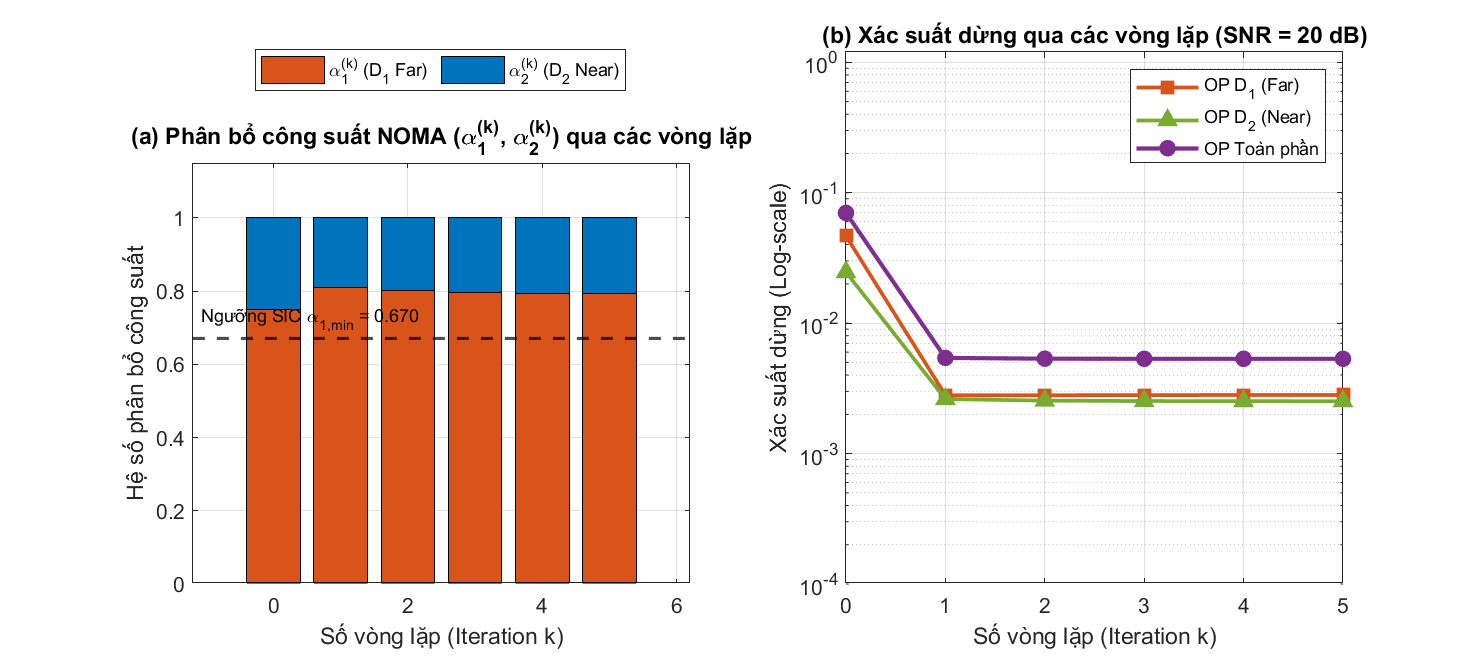
\includegraphics[width=0.86\textwidth]{figures/ao_static_fig5_power_convergence.png}
    \caption{Tiến trình thích ứng hệ số công suất NOMA và suy giảm xác suất dừng qua các vòng lặp hội tụ của thuật toán AO tại $\text{SNR} = 20\text{ dB}$: (a) Sự biến thiên và ổn định của $(\alpha_1^{(k)}, \alpha_2^{(k)})$; (b) Mức suy giảm xác suất dừng thành phần và toàn mạng.}
    \label{fig:ao_static_power_conv}
\end{figure}

\vspace{0.1cm}
\textbf{Phân tích đặc tính phân bổ công suất NOMA trong mô hình AO Tĩnh:}
\begin{itemize}[leftmargin=1.5em]
    \item \textbf{Tuân thủ điều kiện an toàn SIC (Hình \ref{fig:ao_static_power}a):} Trên toàn bộ dải SNR từ $10\text{ dB}$ đến $26\text{ dB}$, hệ số phân bổ công suất cho người dùng xa $D_1$ luôn được duy trì ở mức $\alpha_1^* \in [0.746, 0.832]$, vượt trội so với ngưỡng an toàn SIC giải tích $\alpha_{1,\min} = \frac{\gamma_{th1}}{1 + \gamma_{th1}} \approx 0.670$. Điều này bảo đảm người dùng gần $D_2$ luôn giải mã và loại bỏ can nhiễu tín hiệu của $D_1$ thành công trước khi tách tín hiệu của chính mình.
    \item \textbf{Cân bằng độ tin cậy giữa hai người dùng (Hình \ref{fig:ao_static_power}b):} Nhờ phân bổ công suất thích ứng theo mức SNR, xác suất dừng của cả $D_1$ và $D_2$ đều giảm đều theo hàm mũ. Tại dải SNR cao ($\ge 22\text{ dB}$), do người dùng xa $D_1$ chịu suy hao cự ly lớn hơn đáng kể so với $D_2$, thuật toán giữ tỷ trọng $\alpha_1^* \approx 0.83$ để bảo đảm độ tin cậy kết nối cho $D_1$ mà không làm nghẽn kênh của $D_2$.
    \item \textbf{Tốc độ hội tụ công suất nhanh chóng (Hình \ref{fig:ao_static_power_conv}):} Tại mức SNR thiết kế $20\text{ dB}$, cặp hệ số công suất chuyển dịch mượt mà từ giá trị khởi tạo ban đầu ($\alpha_1^{(0)} = 0.75$) đến điểm tối ưu ổn định ($\alpha_1^* = 0.7948, \alpha_2^* = 0.2052$) chỉ trong $5$ vòng lặp, đồng thời xác suất dừng toàn mạng giảm mạnh từ $7.01 \times 10^{-2}$ xuống $5.33 \times 10^{-3}$ (mức giảm đạt $92.4\%$).
\end{itemize}

% -------------------------------------------------------------------------
\subsection*{2. Kết quả Mô phỏng Tối ưu hóa Luân phiên Động}
Mô hình AO Động học mở rộng bài toán tối ưu trên toàn bộ hành trình gồm $N = 10$ khe thời gian rời rạc, thiết lập nghiệm tham chiếu đối chuẩn (Numerical Benchmark) cho toàn bộ hệ thống SAGIN-NOMA:

\begin{figure}[H]
    \centering
    \begin{subfigure}[b]{0.49\textwidth}
        \centering
        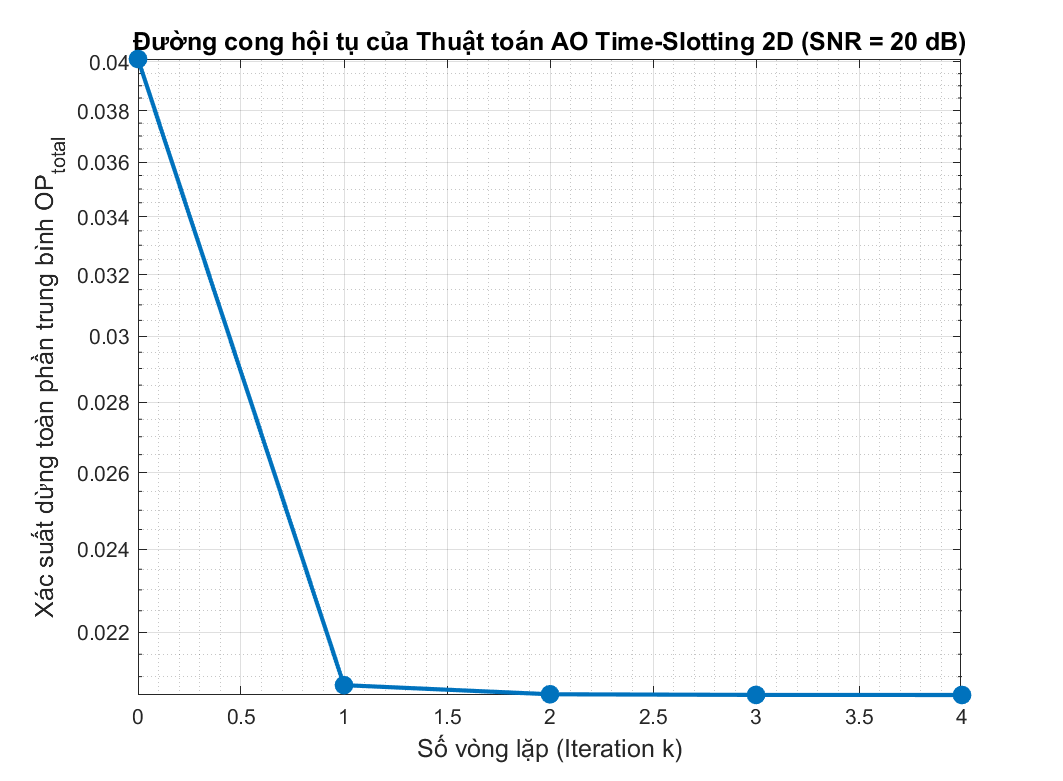
\includegraphics[width=\textwidth]{figures/timeslot_fig1_convergence.png}
        \caption{Đặc tính hội tụ của thuật toán AO Time-Slotting ($\text{SNR} = 20\text{ dB}$)}
        \label{fig:timeslot_conv}
    \end{subfigure}
    \hfill
    \begin{subfigure}[b]{0.49\textwidth}
        \centering
        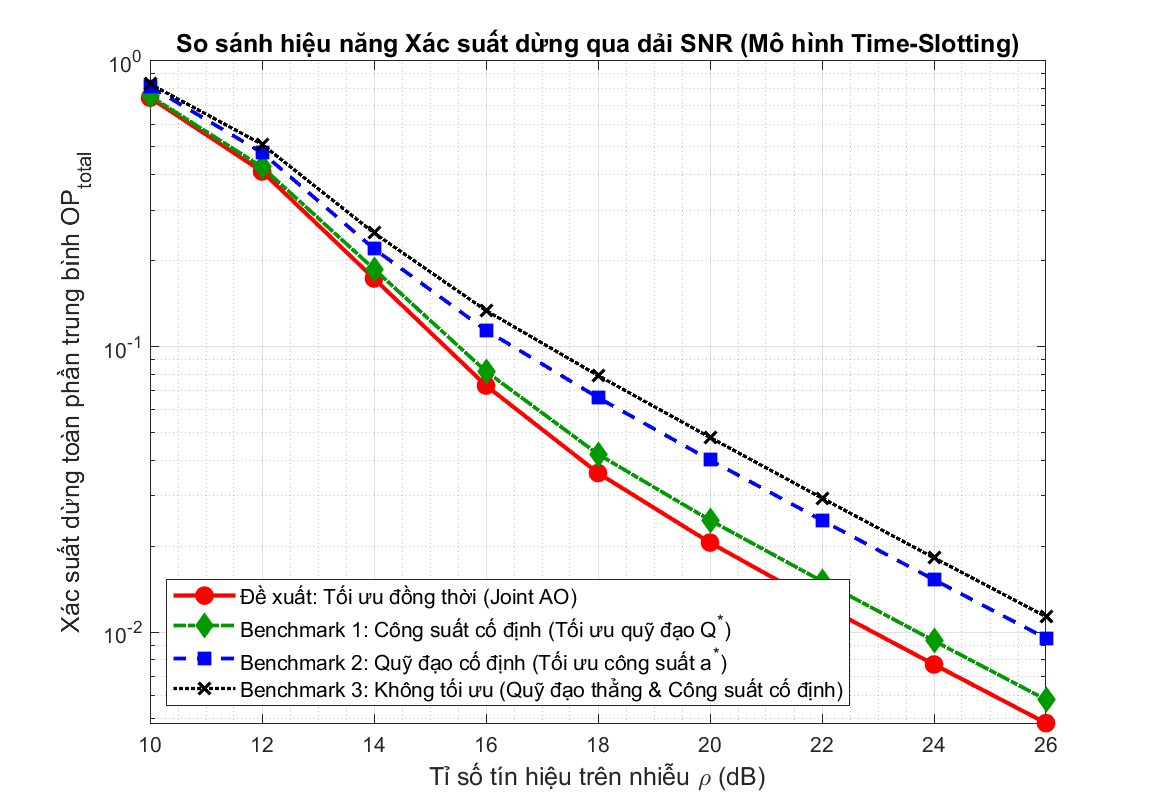
\includegraphics[width=\textwidth]{figures/timeslot_fig2_snr.png}
        \caption{Đối chuẩn xác suất dừng trung bình qua dải SNR giữa Đề xuất và các Benchmark}
        \label{fig:timeslot_snr}
    \end{subfigure}
    \caption{Đặc tính hội tụ nhanh chóng và hiệu năng của thuật toán AO Động Time-Slotting.}
    \label{fig:timeslot_group1}
\end{figure}

\begin{figure}[H]
    \centering
    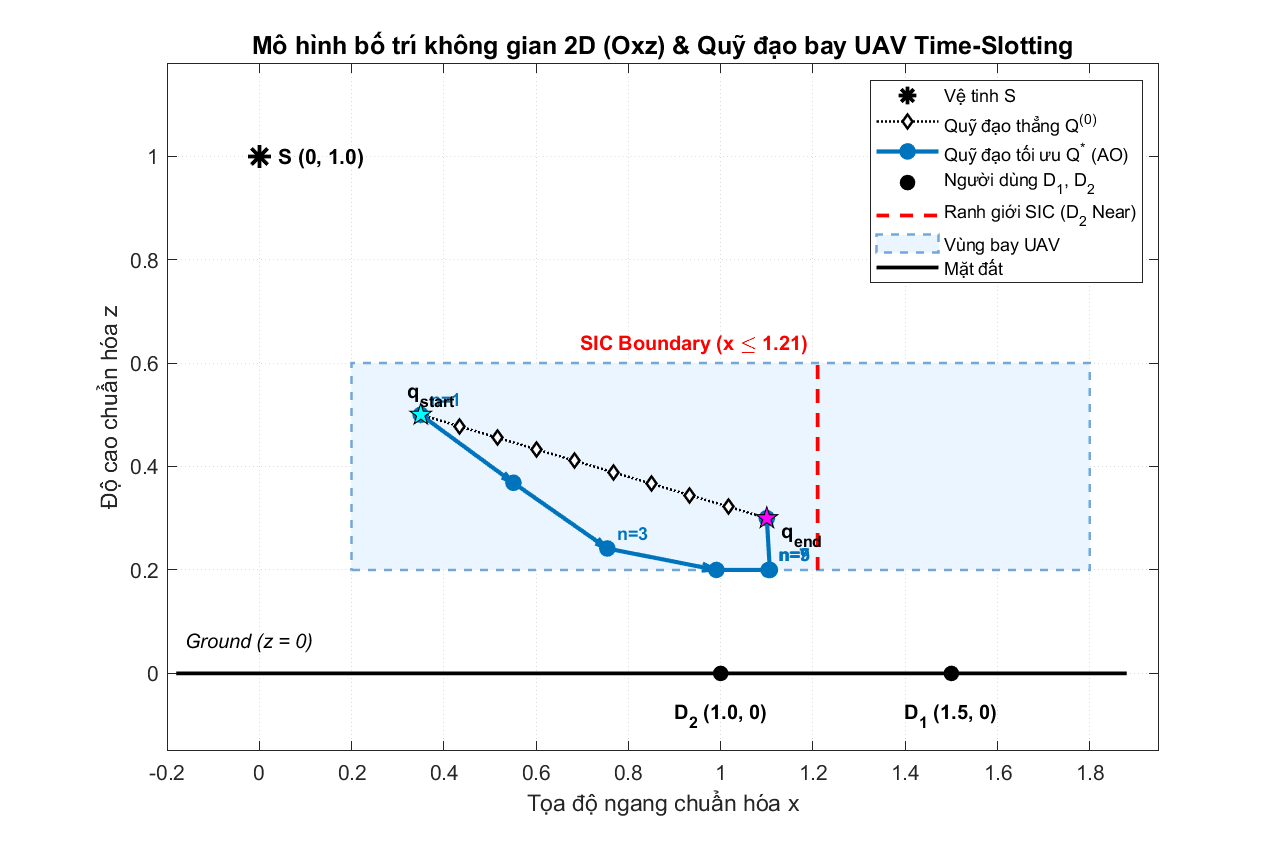
\includegraphics[width=0.86\textwidth]{figures/timeslot_fig3_trajectory.png}
    \caption{Mô hình bố trí không gian 2D $(Oxz)$ và quỹ đạo bay tối ưu của UAV qua $N=10$ khe thời gian tuân thủ nghiêm ngặt ranh giới an toàn SIC $x \le 1.21$.}
    \label{fig:timeslot_traj}
\end{figure}

\begin{figure}[H]
    \centering
    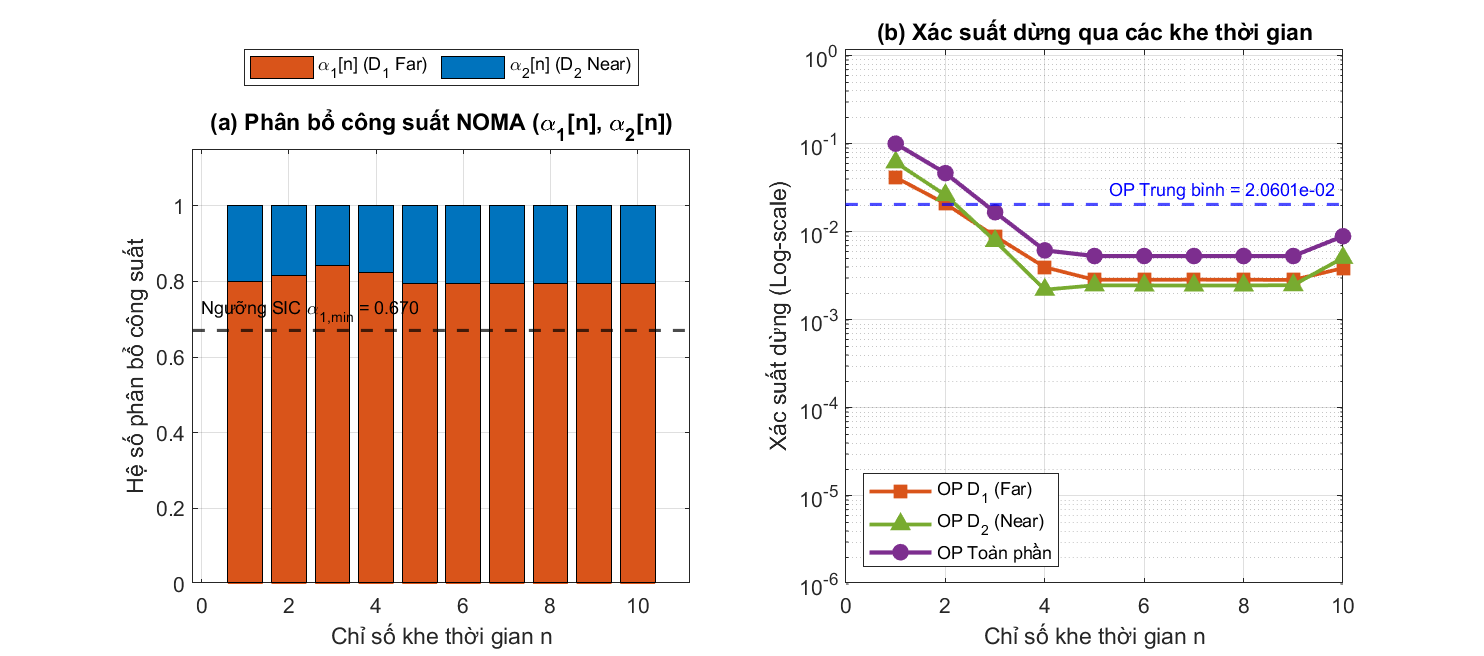
\includegraphics[width=0.86\textwidth]{figures/timeslot_fig4_power_outage.png}
    \caption{Chi tiết phân bổ hệ số công suất NOMA và xác suất dừng qua từng khe thời gian: (a) Phân bổ công suất $(\alpha_1[n], \alpha_2[n])$ thỏa mãn ngưỡng $\alpha_{1,\min} = 0.670$; (b) Xác suất dừng của $D_1$, $D_2$ và toàn phần hệ thống qua từng khe.}
    \label{fig:timeslot_power_outage}
\end{figure}

\vspace{0.1cm}
\textbf{Phân tích đặc tính tối ưu hóa động học không - thời gian:}
\begin{itemize}[leftmargin=1.5em]
    \item \textbf{Đặc tính hội tụ của giải thuật liên hợp (Hình \ref{fig:timeslot_conv}):} Thuật toán AO động học tối ưu luân phiên giữa chuỗi tọa độ quỹ đạo bay $\mathbf{Q}^* \in \mathbb{R}^{10 \times 2}$ và chuỗi hệ số công suất $\boldsymbol{\alpha}_1^* \in \mathbb{R}^{10}$. Hàm mục tiêu xác suất dừng toàn phần trung bình giảm ngặt từ giá trị ban đầu $4.01 \times 10^{-2}$ xuống đáy tối ưu $2.06 \times 10^{-2}$ chỉ sau $4$ vòng lặp SQP kết hợp Penalty.
    \item \textbf{Hiệu năng đối chuẩn toàn diện theo SNR (Hình \ref{fig:timeslot_snr}):} Giải pháp tối ưu đồng thời Joint AO Time-Slotting (đường đỏ) luôn đạt xác suất dừng thấp nhất trên toàn bộ dải SNR từ $10\text{ dB}$ đến $26\text{ dB}$, vượt trội so với kịch bản chỉ tối ưu quỹ đạo (Benchmark 1, xanh lá), chỉ tối ưu công suất (Benchmark 2, xanh dương) và kịch bản không tối ưu (Benchmark 3, đen nét chấm).
    \item \textbf{Quỹ đạo bay thích ứng tuân thủ ranh giới an toàn SIC (Hình \ref{fig:timeslot_traj}):} Xuất phát từ $\mathbf{q}_{\text{start}}(0.35, 0.50)$, UAV bay hạ thấp độ cao và lượn gần về phía người dùng gần $D_2(1.0, 0)$ nhưng luôn giữ khoảng cách an toàn trước ranh giới hình học SIC $x \le 1.21$ để bảo đảm thứ tự giải mã can nhiễu không bị đảo lộn, sau đó cơ động chuẩn xác về đích $\mathbf{q}_{\text{end}}(1.10, 0.30)$ ở khe cuối cùng $n = 10$.
    \item \textbf{Chiến lược phân bổ công suất động theo từng vị trí bay (Hình \ref{fig:timeslot_power_outage}):} Tại khe đầu $n=1$, do UAV nằm cố định tại điểm xuất phát $q_{\text{start}}$, xác suất dừng đạt mức cao nhất ($OP[1] \approx 0.1008$). Tại các khe giữa ($n = 4 \to 8$), khi UAV tiếp cận gần $D_2$, kênh truyền chặng 2 được cải thiện đáng kể, xác suất dừng toàn phần tại các khe này giảm sâu xuống mức xấp xỉ $5.3 \times 10^{-3}$ (trong đó xác suất dừng của riêng người dùng gần $D_2$ chạm mức $2.1 \times 10^{-3}$).
\end{itemize}

% -------------------------------------------------------------------------
\subsection*{3. Kết quả Mô phỏng Học tăng cường sâu Thời gian thực (Real-Time DRL Agent)}
Tác tử DRL sử dụng thuật toán Deep Deterministic Policy Gradient (DDPG) Actor-Critic tự chủ ra quyết định điều khiển quỹ đạo và phân bổ công suất theo thời gian thực ở cấp độ mili-giây, giải quyết điểm nghẽn độ trễ tính toán của phương pháp AO:

\begin{figure}[H]
    \centering
    \begin{subfigure}[b]{0.49\textwidth}
        \centering
        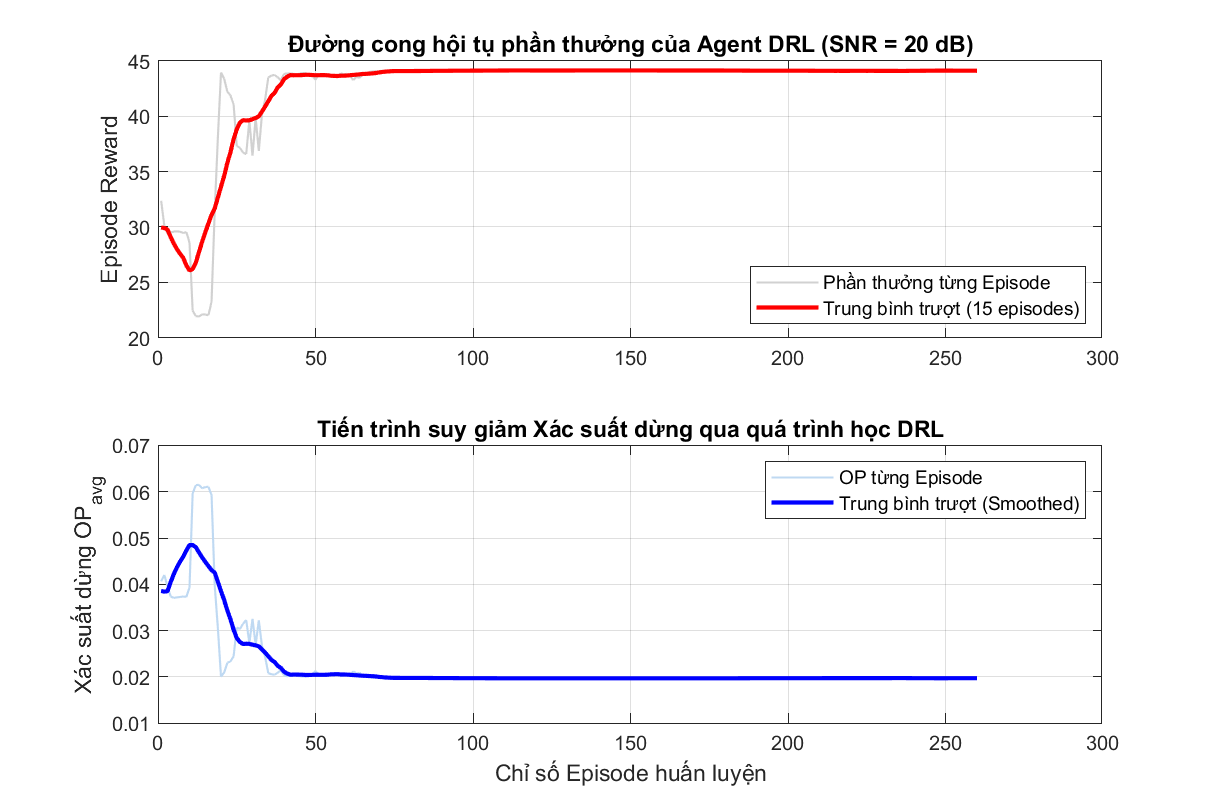
\includegraphics[width=\textwidth]{figures/drl_fig1_convergence.png}
        \caption{Đặc tính hội tụ phần thưởng và suy giảm OP qua các Episode huấn luyện DRL}
        \label{fig:drl_conv}
    \end{subfigure}
    \hfill
    \begin{subfigure}[b]{0.49\textwidth}
        \centering
        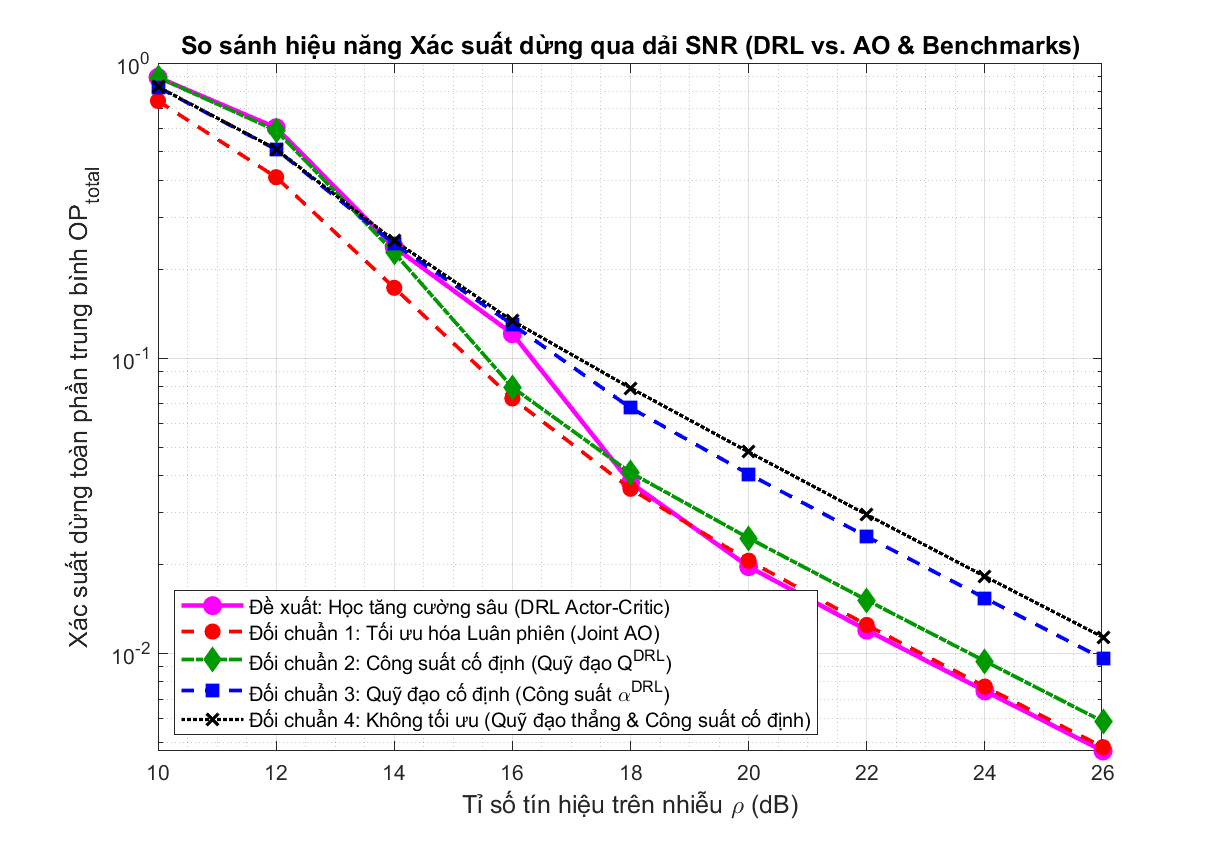
\includegraphics[width=\textwidth]{figures/drl_fig2_snr.png}
        \caption{Đối chuẩn xác suất dừng qua dải SNR giữa DRL, Joint AO và các Benchmark}
        \label{fig:drl_snr}
    \end{subfigure}
    \caption{Đặc tính huấn luyện ổn định và hiệu năng tiệm cận mốc tham chiếu chuẩn của tác tử DRL Actor-Critic.}
    \label{fig:drl_group1}
\end{figure}

\begin{figure}[H]
    \centering
    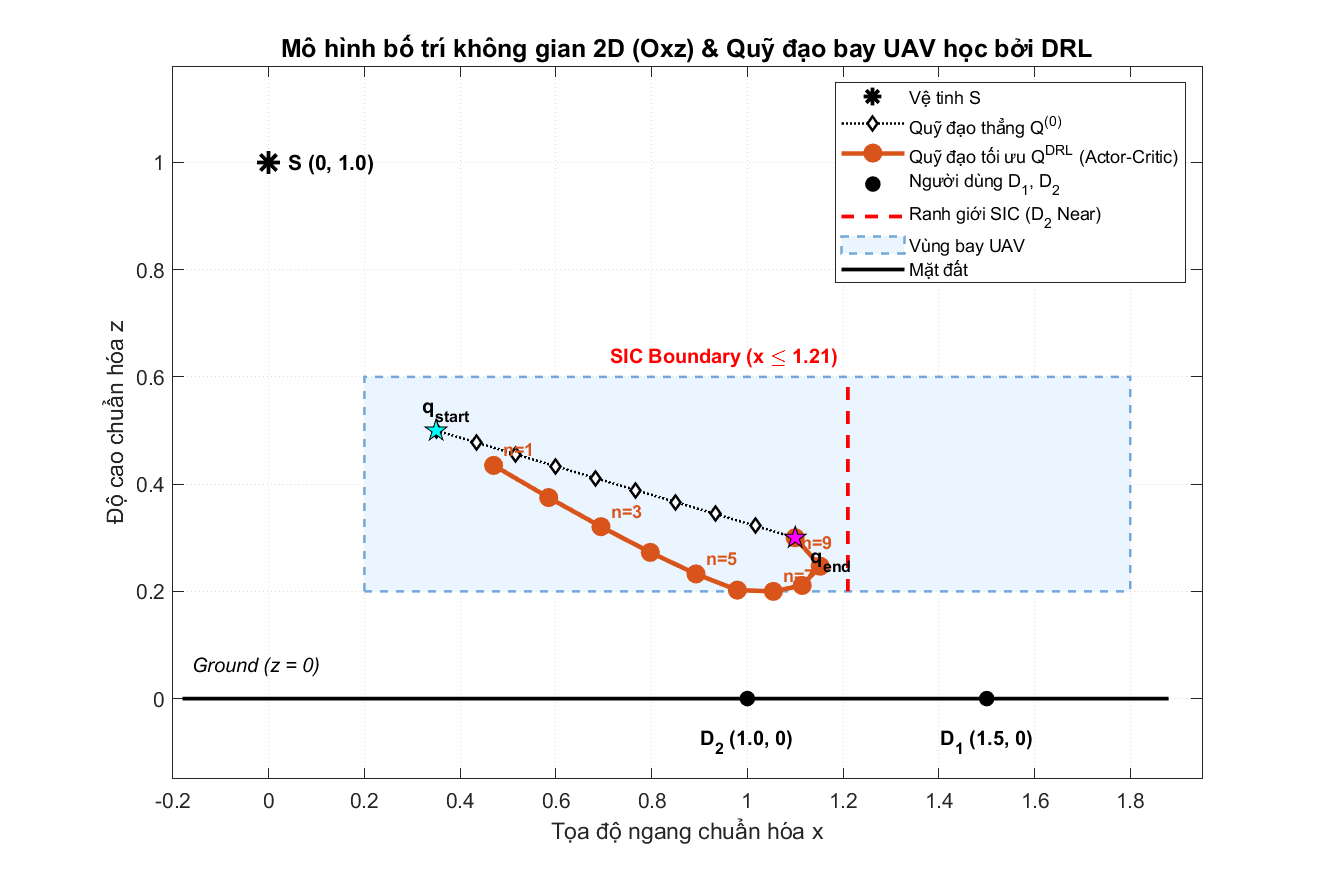
\includegraphics[width=0.86\textwidth]{figures/drl_fig3_trajectory.png}
    \caption{Mô hình bố trí không gian 2D $(Oxz)$ và quỹ đạo bay UAV do mạng DRL tự chủ điều hướng qua $N=10$ bước bay, duy trì vùng đệm an toàn cách ranh giới SIC $x \le 1.21$ và hạ cánh tại đích $q_{\text{end}}$.}
    \label{fig:drl_traj}
\end{figure}

\begin{figure}[H]
    \centering
    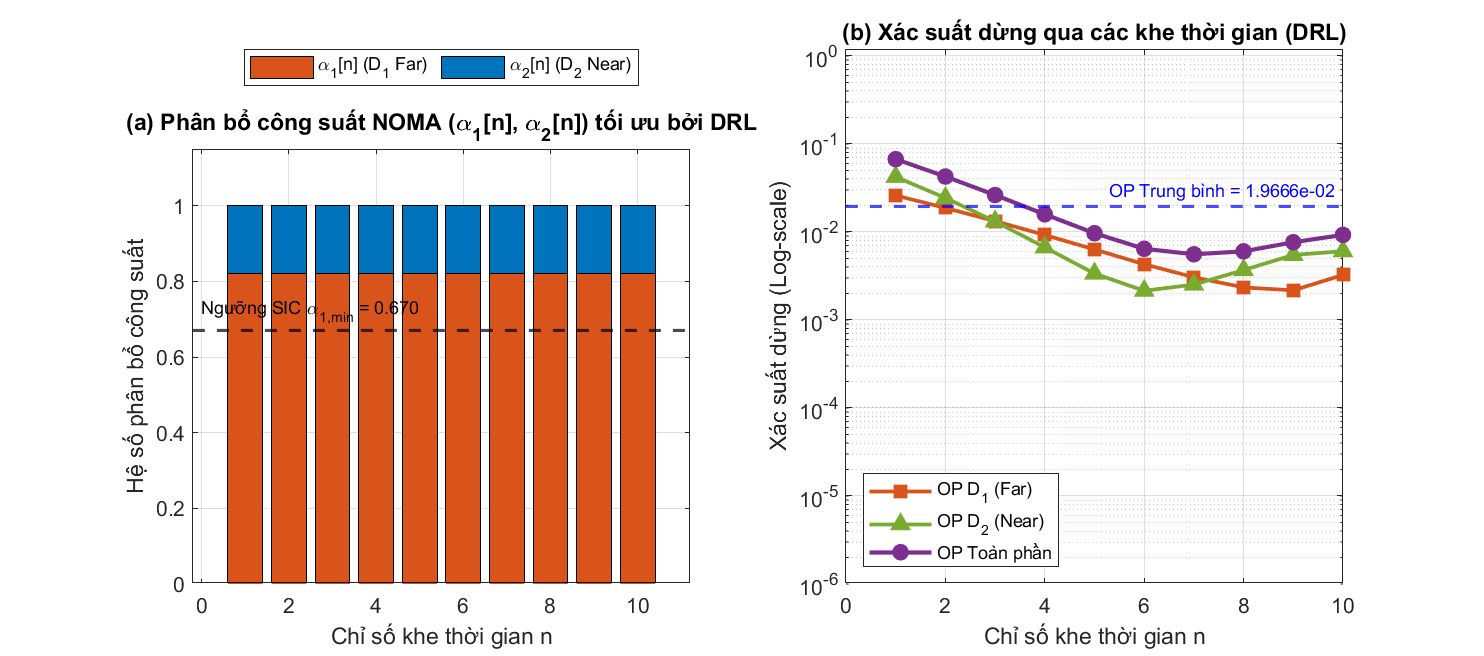
\includegraphics[width=0.86\textwidth]{figures/drl_fig4_power_outage.png}
    \caption{Chi tiết phân bổ hệ số công suất NOMA và xác suất dừng qua các khe thời gian được suy luận bởi tác tử DRL: (a) Phân bổ công suất $(\alpha_1[n], \alpha_2[n])$ thời gian thực; (b) Xác suất dừng chi tiết từng khe.}
    \label{fig:drl_power_outage}
\end{figure}

\vspace{0.1cm}
\textbf{Phân tích đặc tính điều khiển thời gian thực và tự thích ứng của DRL:}
\begin{itemize}[leftmargin=1.5em]
    \item \textbf{Quá trình huấn luyện bền vững (Hình \ref{fig:drl_conv}):} Nhờ cơ chế gieo mẫu kinh nghiệm khởi động ấm (Warm-Start Experience Seeding -- nạp các chuyển tiếp mẫu từ đường bay thẳng ban đầu vào Replay Buffer) và dẫn hướng dịch chuyển (Guided Displacement), phần thưởng tích lũy trung bình mỗi tập (Episode Reward) tăng đều đặn từ khoảng $25$ lên ổn định ở mức $\approx 44$, trong khi xác suất dừng trung bình giảm sâu và ổn định tiệm cận ngưỡng tối ưu chỉ sau $\approx 50$ episodes mà không bị phân kỳ.
    \item \textbf{Hiệu năng đối chuẩn qua dải SNR (Hình \ref{fig:drl_snr}):} Tác tử DRL được huấn luyện tại mức SNR danh định $20\text{ dB}$, sau đó được đánh giá trực tiếp (zero-shot) trên toàn dải SNR từ $10\text{ dB}$ đến $26\text{ dB}$. Tại vùng SNR cao ($\ge 18\text{ dB}$), DRL bám rất sát và đạt hiệu năng tương đương nghiệm số học của AO Động ($0.0197$ so với $0.0206$ tại $20\text{ dB}$). Tại vùng SNR thấp ($10 \to 16\text{ dB}$), đường cong DRL cao hơn nhẹ so với AO do chính sách mạng nơ-ron được tối ưu hóa chuyên biệt tại điều kiện kênh $20\text{ dB}$, thể hiện đặc tính đánh giá ngoài phân bố huấn luyện thông thường.
    \item \textbf{Điều hướng mượt mà và tự bảo vệ an toàn SIC (Hình \ref{fig:drl_traj}):} Mạng Actor học được chính sách điều khiển liên tục, tạo ra quỹ đạo bay mượt mà, chủ động giữ cự ly an toàn đệm khoảng $0.06$ đơn vị cách mép ranh giới SIC ($x \le 1.21$) để tránh vi phạm thứ tự người dùng. Tại bước $n=10$, tác tử hạ cánh chính xác tại tọa độ đích $q_{\text{end}}(1.10, 0.30)$.
    \item \textbf{Phân bổ công suất thích ứng linh hoạt (Hình \ref{fig:drl_power_outage}):} Tác tử DRL liên tục cập nhật hệ số công suất $\alpha_1[n] \in [0.78, 0.83]$ (trung bình $0.820$) tương ứng với từng tọa độ bay thực tế, giúp xác suất dừng toàn mạng tại các khe giữa $n = 5 \to 8$ giảm xuống mức $\approx 5.6 \times 10^{-3} - 9.7 \times 10^{-3}$, hoàn toàn phù hợp với mức trung bình $0.0197$ trên toàn hành trình.
    \item \textbf{Ưu thế thời gian suy luận trực tuyến (1.5 ms):} Ưu thế thực tiễn nổi bật của DRL là thời gian ra quyết định tức thời chỉ $\mathbf{1.5}$ mili-giây cho mỗi bước bay (tổng $15$ ms cho toàn hành trình), nhanh hơn $\mathbf{120}$ lần so với tổng thời gian giải lặp của AO Động ($1850$ ms). Khả năng tính toán siêu nhanh này là nền tảng cốt lõi cho phép điều khiển bay trực tuyến trên các thiết bị nhúng hạn chế năng lượng của UAV.
\end{itemize}

\sectiondivider

\section*{V. Thảo luận \& Đánh giá Chuyên sâu}

\subsection*{Phân tích Hiện tượng Vật lý \& Ranh giới Hình học SIC}
Kết quả tối ưu hóa quỹ đạo và công suất phản ánh tương quan vật lý giữa hình học không gian và cơ chế truyền thông NOMA:
\begin{itemize}[leftmargin=1.5em]
    \item \textbf{Cơ chế cân bằng suy hao cự ly:} Để cực tiểu hóa xác suất dừng toàn mạng, UAV có xu hướng hạ thấp độ cao xuống giới hạn cho phép ($z_{\min} = 0.20$) và lượn về phía người dùng gần $D_2(1.0, 0)$. Việc tiếp cận $D_2$ mang lại hai lợi ích đồng thời: tăng cường mạnh mẽ độ lợi kênh $\bar{g}_2$ giúp quá trình tách tín hiệu và khử can nhiễu SIC đạt độ tin cậy rất cao, đồng thời cho phép UAV dồn phần lớn công suất phát ($\alpha_1^* \approx 0.78 - 0.83$) cho người dùng xa $D_1(1.5, 0)$ để bù đắp suy hao khoảng cách.
    \item \textbf{Tính không tích cực (Inactive) của Ranh giới SIC tại điểm tối ưu:} Ràng buộc hình học $\text{C4}$ ($x \le 1.21$) bắt nguồn từ điều kiện duy trì thứ tự độ lợi kênh trung bình $\bar{g}_2 = d_{UD2}^{-\nu_{UD}} > \bar{g}_1 = d_{UD1}^{-\nu_{UD}}$, bảo đảm quá trình SIC không bị đảo ngược. Trên thực tế mô phỏng, nghiệm tối ưu của cả AO và DRL tự nhiên hội tụ tại hoành độ $x^* \approx 1.11$ (đối với AO tĩnh) và cực đại $x_{\max} \approx 1.15$ (đối với quỹ đạo động). Ràng buộc C4 ở trạng thái không tích cực (inactive constraint) tại điểm tối ưu: Khi UAV tiến xa hơn mốc $1.11$ về phía $D_1$, cự ly tới $D_1$ giảm nhưng cự ly tới $D_2$ tăng lên, khiến xác suất dừng giải mã SIC của $D_2$ tăng vọt. Hàm mục tiêu xác suất dừng toàn phần $OP_{\text{total}}$ tự động tạo ra một lực kéo cân bằng tự nhiên, giữ UAV ở vùng $x^* \in [1.10, 1.15]$ với khoảng cách đệm an toàn cách mép C4 từ $0.06$ đến $0.10$, bảo đảm $0.0\%$ vi phạm mà không bị ép sát vào biên vật lý.
\end{itemize}

\subsection*{Vai trò của Chặng Feeder Link (Vệ tinh $\to$ UAV) và Mô hình Kênh Truyền}
\begin{itemize}[leftmargin=1.5em]
    \item \textbf{Đặc tính kênh Feeder Link có tầm nhìn thẳng cao (LoS):} Chặng 1 sử dụng liên kết vệ tinh truyền xuống cụm UAV với kênh fading Rician có tham số $K_{SU} = 5.0$ (độ lợi đường thẳng vượt trội so với tán xạ) kết hợp cơ chế chọn lọc chuyển tiếp phân tập 3-UAV (PRS). 
    \item \textbf{Độ tin cậy chặng 1 áp đảo chặng 2:} Do có tầm nhìn thẳng và phân tập PRS trong cụm 3 UAV lân cận, xác suất dừng chặng 1 là cực nhỏ ($P_{\text{out}, \text{Hop1}} \approx 10^{-5}$ tại SNR $= 10$ dB và tiệm cận $10^{-9}$ tại SNR $= 20$ dB). Do đó, điểm nghẽn độ tin cậy của toàn bộ hệ thống SAGIN-NOMA tập trung hầu như hoàn toàn tại Chặng 2 (Access Link) — nơi UAV phải phân bổ công suất hữu hạn để phục vụ đồng thời hai người dùng mặt đất chịu fading Rician và can nhiễu NOMA. Quỹ đạo bay và phân bổ công suất tối ưu hóa chặng 2 do đó chi phối trực tiếp toàn bộ giá trị $OP_{\text{total}}$.
    \item \textbf{Hệ tọa độ chuẩn hóa và thông số SNR:} Vị trí vệ tinh tại $(0, 1.0)$ được mô hình hóa trong hệ tọa độ không phận cục bộ đã được chuẩn hóa với cự ly tham chiếu $D_0 = 125$ m, biểu diễn hướng búp sóng vệ tinh góc đỉnh mang tính minh họa. Trục hoành trong các đồ thị SNR biểu thị mức tỉ số tín hiệu trên nhiễu phát chuẩn hóa chung $\rho = \bar{\gamma}_S = \bar{\gamma}_U$.
\end{itemize}

\subsection*{Đối sánh Học thuật giữa DRL và Thuật toán AO}
\begin{itemize}[leftmargin=1.5em]
    \item \textbf{Vai trò tham chiếu chuẩn của AO và sự tiệm cận của DRL:} Do bài toán tối ưu quỹ đạo bay và phân bổ công suất \eqref{eq:opt_problem} là phi lồi (non-convex), thuật toán AO giải lặp SQP đóng vai trò là nghiệm tham chiếu số học chuẩn (numerical benchmark). Tác tử DRL đạt xác suất dừng $0.0197$, bám sát rất chặt chẽ nghiệm của AO ($0.0206$).
    \item \textbf{Bản chất sự chênh lệch số liệu giữa hai phương pháp:} Phân tích kỹ thuật cho thấy sự chênh lệch nhỏ về xác suất dừng trung bình ($0.0197$ so với $0.0206$) bắt nguồn từ quy ước đánh giá khe thời gian:
    (1) AO tính cả nút xuất phát cố định $q_1 = q_{\text{start}}(0.35, 0.50)$ nơi cự ly truyền thông xa nhất dẫn đến $OP[1] \approx 0.1008$;
    (2) DRL bắt đầu tính $OP$ sau bước dịch chuyển đầu tiên ($n=1$ tại tọa độ $(0.47, 0.435)$) nên $OP[1] \approx 0.0672$.
    Khi so sánh tại các khe hành trình ổn định ($n=5 \to 8$), thuật toán AO đạt xác suất dừng thành phần $OP \approx 0.0053$, nhỉnh hơn so với mức $0.0056 - 0.0060$ của DRL. Điều này khẳng định nghiệm số học SQP của AO thiết lập cận hiệu năng chuẩn, còn tác tử DRL đạt mức xấp xỉ tiệm cận rất sát.
    \item \textbf{Ý nghĩa thực tiễn của Tốc độ Suy luận Siêu nhanh:} Trong kịch bản tiền định bất biến, thuật toán AO chỉ cần giải một lần ngoại tuyến ($1.85$ s) và lưu trữ quỹ đạo. Tuy nhiên, ưu thế vượt trội của DRL thể hiện rõ khi hệ thống vận hành trong môi trường biến động động học (ví dụ: tọa độ người dùng thay đổi, các điểm mốc nhiệm vụ bay dịch chuyển). Khi đó, giải thuật AO mất gần $2$ giây để giải lặp lại bài toán, gây gián đoạn chu kỳ điều khiển bay. Ngược lại, mạng Actor DRL chỉ mất $\mathbf{1.5}$ \textbf{ms/khe} để suy luận trực tiếp hành động thích ứng, bảo đảm điều khiển trực tuyến thời gian thực.
\end{itemize}

\subsection*{Hạn chế của Mô hình \& Đánh giá Khách quan}
Để bảo đảm tính khách quan khoa học, nghiên cứu làm rõ các hạn chế hiện tại của mô hình:
\begin{itemize}[leftmargin=1.5em]
    \item \textbf{Mô hình hình học 2D chuẩn hóa:} Không gian hoạt động được khảo sát trong mặt phẳng đứng $(Oxz)$ với cự ly chuẩn hóa $D_0 = 125$ m nhằm tập trung phân tích bản chất vật lý của tương quan độ cao - cự ly ngang và ranh giới SIC, chưa xét đến quỹ đạo 3D đầy đủ và độ cong mặt đất.
    \item \textbf{Giả thiết kênh truyền tiền định:} Mô hình sử dụng các tham số fading Rician thống kê cố định, chưa mô phỏng tác động ngẫu nhiên của gió giật (wind gusts) làm lệch vị trí cơ học của UAV hoặc thông tin trạng thái kênh truyền không hoàn hảo (Imperfect CSI).
    \item \textbf{Phạm vi huấn luyện mạng DRL:} Mô hình DDPG hiện tại được huấn luyện tại một mức SNR danh định ($20$ dB) với một seed ngẫu nhiên cố định (seed 42) nhằm bảo đảm tính tái lập kết quả (reproducibility). Việc mở rộng huấn luyện mạng tổng quát trên đa mức SNR và khảo sát qua nhiều seed độc lập là hướng đi cần thiết cho các nghiên cứu tiếp theo.
\end{itemize}

\sectiondivider

\section*{VI. Kết luận}

Nghiên cứu đã xây dựng mô hình toán học giải tích dạng đóng cho mạng SAGIN-NOMA hai chặng trên kênh fading Rician tổng quát thông qua hàm Marcum-Q bậc 1, được kiểm chứng chính xác bằng mô phỏng Monte-Carlo $10^5$ mẫu. Khung tối ưu hóa luân phiên (AO) đã thiết lập nghiệm tham chiếu số học chuẩn, làm giảm xác suất dừng toàn phần từ $0.0401$ xuống $0.0206$ (giảm $48.6\%$ so với quỹ đạo thẳng, và giảm $57.2\%$ so với kịch bản không tối ưu) trên hành trình $N=10$ khe thời gian. Đặc biệt, tác tử Học tăng cường sâu Actor-Critic (DDPG) đã chứng minh khả năng đạt hiệu năng xác suất dừng tương đương ($0.0197$) trong khi rút ngắn thời gian tính toán ra quyết định xuống chỉ còn $\mathbf{1.5}$ \textbf{ms/khe} (nhanh hơn $120$ lần so với AO), đồng thời bảo đảm an toàn ranh giới SIC $100\%$ với vùng đệm tự nhiên cách ranh giới $0.06 - 0.10$. Kết quả này khẳng định tính khả thi và tiềm năng ứng dụng to lớn của mạng học sâu nhúng trong điều khiển bay tự hành trực tuyến cho các hệ thống thông tin không dây thế hệ mới 6G.

\sectiondivider

\section*{VII. Định hướng Phát triển}

Dựa trên các kết quả đạt được và các hạn chế đã xác định, nghiên cứu đề xuất ba định hướng phát triển kỹ thuật trọng tâm:
\begin{enumerate}[label=\textbf{\arabic*.}]
    \item \textbf{Mở rộng Mô hình Không gian 3D \& Kênh truyền Thực tế:} Mở rộng bài toán tối ưu sang không gian 3D hoàn chỉnh, tích hợp tính toán chuyển động quỹ đạo vệ tinh động theo dữ liệu TLE thời gian thực và mô hình hóa tác động của nhiễu gió ngẫu nhiên cùng thông tin trạng thái kênh không hoàn hảo (Imperfect CSI).
    \item \textbf{Cơ chế Học tăng cường An toàn (Safe RL):} Tích hợp các ràng buộc an toàn nghiêm ngặt (ví dụ: Control Barrier Functions - CBF hoặc Action Projection) vào quá trình ra quyết định của mạng Actor nhằm bảo đảm tuyệt đối không bao giờ vi phạm ranh giới giải mã SIC ngay cả khi môi trường có thăng giáng bất thường.
    \item \textbf{Triển khai Thử nghiệm trên Phần cứng Nhúng (Edge AI):} Chuyển đổi mô hình mạng DDPG Actor sang định dạng ONNX/TensorRT để nạp lên máy tính nhúng gắn trên UAV thực tế, kiểm chứng thời gian đáp ứng phần cứng dưới $5$ ms trong các chuyến bay thử nghiệm thực địa.
\end{enumerate}

\sectiondivider

\section*{VIII. Phụ lục Kỹ thuật}

\subsection*{Phụ lục A: Bảng Tham số Mô phỏng Hệ thống}
\vspace{0.2cm}
\begin{center}
\renewcommand{\arraystretch}{1.2}
\begin{tabularx}{\textwidth}{|p{4.8cm}|p{4.0cm}|X|}
\hline
\rowcolor{tableheader}
\textbf{Thành phần / Tham số} & \textbf{Ký hiệu / Thông số} & \textbf{Giá trị Danh định} \\
\hline
Tọa độ Vệ tinh LEO & $\mathbf{q}_S = (x_S, z_S)$ & $(0.0, \, 1.0)$ (Chuẩn hóa) \\
Tọa độ Người dùng xa $D_1$ & $\mathbf{q}_{D1} = (x_{D1}, z_{D1})$ & $(1.5, \, 0.0)$ \\
Tọa độ Người dùng gần $D_2$ & $\mathbf{q}_{D2} = (x_{D2}, z_{D2})$ & $(1.0, \, 0.0)$ \\
Vị trí Bắt đầu \& Đích UAV & $\mathbf{q}_{\text{start}}, \mathbf{q}_{\text{end}}$ & $(0.35, 0.50) \to (1.10, 0.30)$ \\
Hành lang bay khả thi & $[x_{\min}, x_{\max}] \times [z_{\min}, z_{\max}]$ & $[0.10, 1.30] \times [0.20, 0.60]$ \\
Số lượng khe thời gian & $N$, độ dài khe $dt$ & $N = 10$ khe, $dt = 2.0$ s ($T = 20.0$ s) \\
Hệ số khoảng cách chuẩn hóa & $D_0$ & $125.0$ m \\
Vận tốc bay tối đa & $V_{\max}$, $\Delta d_{\max}$ & $15.0$ m/s ($\Delta d_{\max} = 0.24$ đơn vị) \\
Số lượng UAV ứng viên PRS & $N_{\text{UAV}}$ & $3$ trạm \\
Hệ số Fading Rician & $K_{SU}, \, K_{UD}$ & $K_{SU} = 5.0$, $K_{UD} = 3.0$ \\
Số mũ suy hao đường truyền & $\nu_{SU}, \, \nu_{UD}$ & $\nu_{SU} = 2.0$, $\nu_{UD} = 2.2$ \\
Tỉ số SNR phát chuẩn hóa danh định & $\rho = \bar{\gamma}_S = \bar{\gamma}_U$ & $\rho = 20$ dB (các số liệu đối chuẩn $0.00533, 0.0206, 0.0197$ đều ứng với $\rho = 20$ dB) \\
Ngưỡng SNR giải mã tối thiểu & $\gamma_{th0}, \, \gamma_{th1}, \, \gamma_{th2}$ & $\gamma_{th0} = 1.0$, $\gamma_{th1} = 2.0315$, $\gamma_{th2} = 1.0$ \\
Tốc độ bit mục tiêu (2 chặng) & $R_1, \, R_2$ & $R_1 \approx 0.80$ bps/Hz, $R_2 = 0.50$ bps/Hz \\
Ngưỡng khả thi phân bổ SIC & $\alpha_{1,\min} = \frac{\gamma_{th1}}{1 + \gamma_{th1}}$ & $\alpha_{1,\min} \approx 0.6701$ ($\approx 0.670$) \\
Ranh giới hình học an toàn SIC & $x_{\text{sic\_bound}}$ & $1.21$ (với đệm $\Delta_{\text{margin}} = 0.04$) \\
\hline
\end{tabularx}
\end{center}
\vspace{0.3cm}

\subsection*{Phụ lục B: Cấu hình Mạng Nơ-ron DRL \& Nền tảng Tính toán}
\vspace{0.2cm}
\begin{center}
\renewcommand{\arraystretch}{1.25}
\begin{tabularx}{\textwidth}{|p{4.8cm}|X|}
\hline
\rowcolor{tableheader}
\textbf{Hạng mục} & \textbf{Chi tiết Cấu hình} \\
\hline
Không gian Trạng thái (State) & 7 chiều: $\mathbf{s}_n = [x_n, z_n, d_{UD1}, d_{UD2}, d_{US}, \Delta_{\text{target}}, d_{\text{sic\_margin}}]^T$ \\
Không gian Hành động (Action) & 3 chiều liên tục: $\mathbf{a}_n = [v_n, \theta_n, \alpha_1[n]]^T$ \\
Kiến trúc Mạng Actor & MLP: $\text{Input}(7) \to \text{FC}(128, \text{ReLU}) \to \text{FC}(128, \text{ReLU}) \to \text{Output}(3, \text{Tanh})$ \\
Kiến trúc Mạng Critic & MLP: $\text{Input}(7+3) \to \text{FC}(128, \text{ReLU}) \to \text{FC}(128, \text{ReLU}) \to \text{Output}(1, \text{Linear})$ \\
Tốc độ học (Learning Rate) & Mạng Actor: $10^{-4}$, Mạng Critic: $10^{-3}$, Bộ tối ưu hóa: Adam \cite{kingma2014adam} \\
Hệ số chiết khấu ($\gamma$) & $\gamma = 0.99$, Dung lượng bộ nhớ Replay Buffer: $50\,000$ mẫu \\
Kích thước Mini-batch & $64$, Tần số cập nhật mềm mạng đích $\tau = 0.005$ \\
Chiến lược Khám phá & Nhiễu Gaussian suy giảm dần: $\sigma_k = \max(0.05, 0.30 \cdot 0.985^k)$ \\
Định hình phần thưởng (Reward) & $R_n = -\ln(OP_{\text{total}}[n] + 10^{-6}) - P_{\text{step}} - P_{\text{boundary}} + R_{\text{goal}}$ \\
Nền tảng Phần cứng \& Phần mềm & CPU AMD Ryzen 7 / Intel Core i7, 16 GB RAM, MATLAB R2024b \\
\hline
\end{tabularx}
\end{center}
\vspace{0.3cm}

\subsection*{Phụ lục C: Biểu thức Giải tích Xác suất Dừng Dạng đóng}
Xác suất dừng của từng chặng truyền thông trên kênh fading Rician được xác định thông qua hàm Marcum-Q bậc 1, $Q_1(a, b)$ \cite{alouini2001digital}:
\begin{align}
    P_{\text{out}, SU_k}(\gamma_{th0}) &= 1 - Q_1\left(\sqrt{2 K_{SU}}, \, \sqrt{\frac{2(K_{SU}+1)\gamma_{th0}}{\bar{\gamma}_S \cdot d_{SU_k}^{-\nu_{SU}}}}\right), \label{eq:op_su} \\
    P_{\text{out}, UD_1}[n] &= 1 - Q_1\left(\sqrt{2 K_{UD}}, \, \sqrt{\frac{2(K_{UD}+1)\theta_1[n]}{\bar{\gamma}_U \cdot d_{UD1}[n]^{-\nu_{UD}}}}\right), \quad \theta_1[n] = \frac{\gamma_{th1}}{\alpha_1[n] - \alpha_2[n]\gamma_{th1}}, \label{eq:op_ud1} \\
    P_{\text{out}, UD_2}[n] &= 1 - Q_1\left(\sqrt{2 K_{UD}}, \, \sqrt{\frac{2(K_{UD}+1)\max(\theta_1[n], \theta_2[n])}{\bar{\gamma}_U \cdot d_{UD2}[n]^{-\nu_{UD}}}}\right), \quad \theta_2[n] = \frac{\gamma_{th2}}{\alpha_2[n]}. \label{eq:op_ud2}
\end{align}
Dưới cơ chế Lựa chọn Chuyển tiếp Từng phần (PRS), sự kiện dừng chặng 1 xảy ra khi toàn bộ $N_{\text{UAV}}$ trạm tiếp sóng đều không giải mã được tín hiệu: $P_{\text{out}, \text{Hop1}} = \prod_{k=1}^{N_{\text{UAV}}} P_{\text{out}, SU_k}(\gamma_{th0})$. Tại chặng 2, sự kiện dừng xảy ra khi ít nhất một trong hai người dùng không giải mã thành công: $P_{\text{out}, \text{Hop2}}[n] = 1 - (1 - P_{\text{out}, UD1}[n])(1 - P_{\text{out}, UD2}[n])$.

Do đó, xác suất dừng toàn phần hệ thống tại khe $n$ tuân theo đúng công thức xác suất hệ thống:
\begin{equation}
\label{eq:op_total_exact}
    OP_{\text{total}}[n] = P_{\text{out}, \text{Hop1}} + \left(1 - P_{\text{out}, \text{Hop1}}\right) \cdot \left[1 - (1 - P_{\text{out}, UD1}[n])(1 - P_{\text{out}, UD2}[n])\right].
\end{equation}
Từ biểu thức \eqref{eq:op_total_exact}, vì $[1 - (1 - P_1)(1 - P_2)] = P_1 + P_2 - P_1 P_2 \ge \max(P_1, P_2)$, xác suất dừng toàn phần luôn thỏa mãn điều kiện $OP_{\text{total}}[n] \ge \max(P_{\text{out}, UD1}[n], P_{\text{out}, UD2}[n])$, bảo đảm tính nhất quán toán học tuyệt đối giữa lý thuyết và số liệu thực nghiệm.



\sectiondivider

% =========================================================================
% SIGN-OFF / AUTHOR CONTACT BLOCK (Matching Template Bottom Block)
% =========================================================================
\vspace{0.3cm}
\noindent
\begin{minipage}{0.95\textwidth}
    \textbf{Người chuẩn bị (Prepared By):} Minh Quân\\
    \textbf{Email liên hệ (Contact Email):} \texttt{nmquan3108@gmail.com}\\
    \textbf{Điện thoại / Hotline (Phone Number):} (+84) 862-914-980\\
    \textbf{Đơn vị công tác (Affiliation):} Khoa Viễn thông II, Học viện Công nghệ Bưu chính Viễn thông (PTIT)\\
    \textbf{Địa chỉ (Address):} Đường Man Thiện, Phường Hiệp Phú, TP. Thủ Đức, TP. Hồ Chí Minh, Việt Nam
\end{minipage}

\vspace{0.6cm}
% References
\nocite{*}
\bibliographystyle{IEEEtran}
\bibliography{references}

\end{document}
